\documentclass[notheorems,hidelinks,aspectratio=1610]{beamer}
%\usetheme[compress]{JuanLesPins}
\usetheme{JuanLesPins}
\usecolortheme{iwr}
\usepackage{mathsim}
\lstset{language=Python}
\usetikzlibrary{snakes}
\usetikzlibrary{matrix,fit}
\pgfdeclarelayer{bg}
\pgfsetlayers{bg,main}
\input{mixed/fig/tikzsettings}
\def\esp#1{V_{#1}}

\usepackage{times}
\usepackage{xr}
\externaldocument{main}
\usepackage{mfirstuc}
\usepackage{mathtools}  
\mathtoolsset{showonlyrefs}

\newcommand{\rd}{\operatorname{rd}}
\definecolor{mygreen}{RGB}{0,160,0}

\def\footnote#1{}
\def\putindex#1{#1}
\title{Differentialgleichungen}
\author{Guido Kanschat}
\date{\today}

\begin{document}
\frame{\maketitle}
\frame{\frametitle{Overview}\tableofcontents[hideallsubsections]}

\section{Modelierung von Populationen}
\frame{\sectoc}
\subsection{Wachstum unter Idealbedingungen}
\frame{\subtoc}
\begin{frame}{Ausgangsfragestellung}
  \begin{columns}
    \begin{column}{.6\textwidth}
      \begin{itemize}
      \item<+-> Anzucht von Hefe
      \item<+-> Fermenter
      \item<+-> Fragen:
        \begin{itemize}
        \item<+-> Wie lange muss ich warten, bis ich die gewünschte Ausbeute habe?
        \item<+-> Kann ich für einen beliebigen Zeitpunkt die Anzahl
          an Hefezellen vorhersagen?
        \end{itemize}
      \end{itemize}
    \end{column}
    \begin{column}{.39\textwidth}
      \begin{center}
        \only<2->{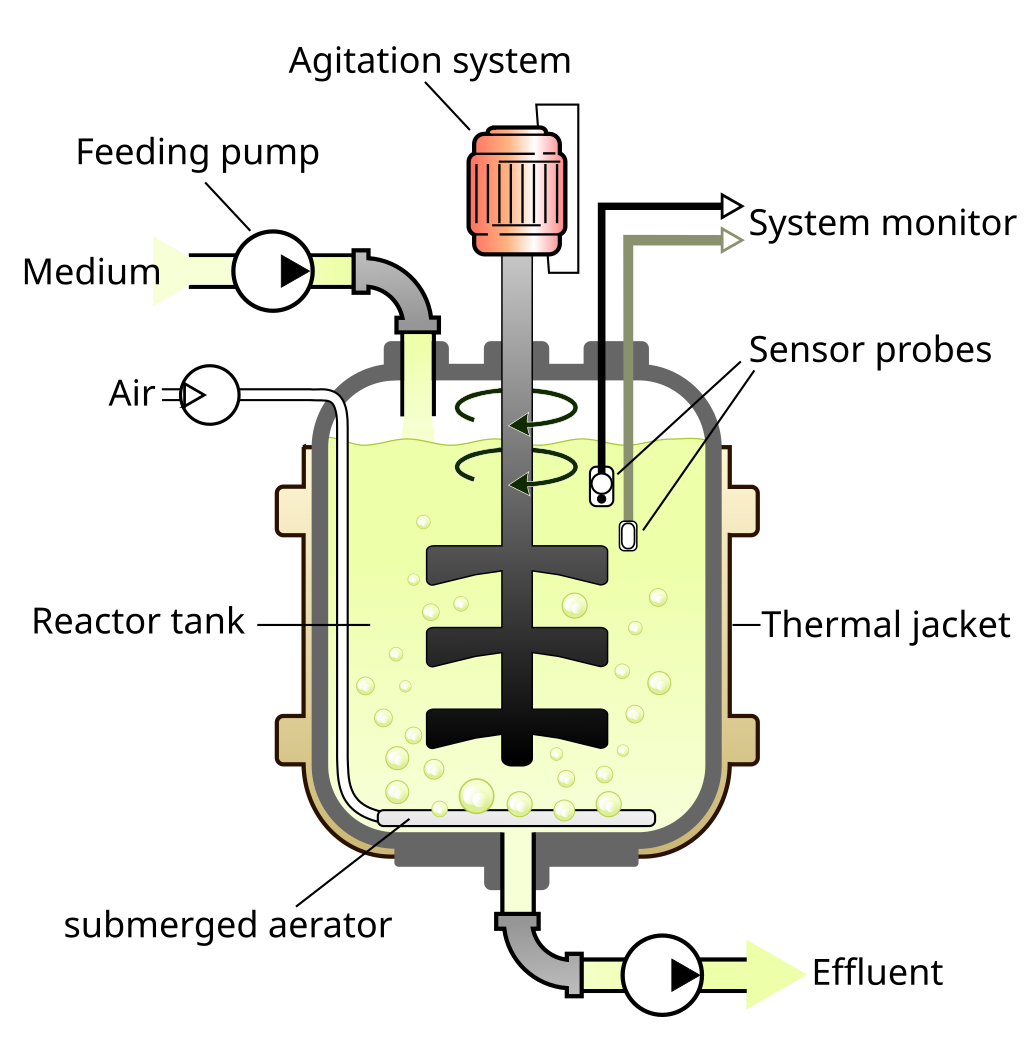
\includegraphics[width=.9\textwidth]{fig/Bioreactor}

          \tiny © Yassine Mrabet, Wikipedia
        }
      \end{center}
    \end{column}
  \end{columns}
\end{frame}

\begin{frame}
  \begin{exampleblock}{Frage}
    Welche Informationen benötigen Sie, um diese Aufgabe zu lösen?
  \end{exampleblock}
\end{frame}

\begin{frame}
  \begin{block}{Verdopplungsrate}
    Under optimal conditions, yeast cells can double their population every 100 minutes.

    \begin{flushright}
      \tiny Wikipedia: Saccaromyces cerevisiæ
    \end{flushright}
  \end{block}

  \pause
  \vspace{5mm}
  
  \begin{tikzpicture}\footnotesize
    \draw [->] (0,0) -- (12.5,0);
    \draw (0,.1)  -- (0,-.1) node[below] {8:00};
    \draw (2,.1) -- (2,-.1) node[below] {9:40};
    \draw (4,.1) -- (4,-.1) node[below] {11:20};
    \draw (6,.1) -- (6,-.1) node[below] {13:00};
    \draw (8,.1) -- (8,-.1) node[below] {14:40};
    \draw (10,.1) -- (10,-.1) node[below] {16:20};
    \draw (12,.1) -- (12,-.1) node[below] {18:00};
    \only<2>{
      \path (1,.3) node {2x};
      \path (3,.3) node {2x};
      \path (5,.3) node {2x};
      \path (7,.3) node {2x};
      \path (9,.3) node {2x};
      \path (11,.3) node {2x};
    }
    \only<3->{
      \path (0.,.1) node[above,iwrred]{1000};
      \path (2.,.1) node[above,iwrred]{2000};
      \path (4.,.1) node[above,iwrred]{4000};
      \path (6.,.1) node[above,iwrred]{8000};
      \path (8.,.1) node[above,iwrred]{16000};
      \path (10.,.1) node[above,iwrred]{32000};
      \path (12.,.1) node[above,iwrred]{64000};
    }
    \only<4>{
      \draw[mygreen] (7,.1) -- (7,-.1) node[below,mygreen] {13:50};
    }
  \end{tikzpicture}

  \pause
  \vspace{5mm}

  \begin{block}{Anfangspopulation}
    Beispiel: Die Population um 8:00 beträgt 1000 Zellen
  \end{block}
  \pause
  \begin{exampleblock}{Frage}
    Wieviele Zellen haben wir um 13:50?
  \end{exampleblock}
\end{frame}

\begin{frame}{Mathematisch etwas allgemeiner und präziser...}
  \begin{itemize}
  \item Anzahlvariable $N$
  \item Zeitvariable $t$ in Minuten, Startzeit $t_0=8:00$, ``Messzeit'' $T=18:00$
  \item Zeitintervalle $I_k = [t_{k-1},t_k]$ der Länge $\Delta t = 100 \text{min}$
    
    \vspace{5mm}
  \begin{tikzpicture}\footnotesize
    \draw [->] (0,0) -- (12.5,0);
    \draw (0,.1)  -- (0,-.1) node[below] {8:00};
    \draw (2,.1) -- (2,-.1) node[below] {9:40};
    \draw (4,.1) -- (4,-.1) node[below] {11:20};
    \draw (6,.1) -- (6,-.1) node[below] {13:00};
    \draw (8,.1) -- (8,-.1) node[below] {14:40};
    \draw (10,.1) -- (10,-.1) node[below] {16:20};
    \draw (12,.1) -- (12,-.1) node[below] {18:00};
      \path (0.,.1) node[above,iwrred]{1000};
      \path (1,.3) node {+1000};
      \path (3,.3) node {+2000};
      \path (5,.3) node {+4000};
      \path (7,.3) node {+8000};
      \path (9,.3) node {+16000};
      \path (11,.3) node {+32000};
    \end{tikzpicture}

    \vspace{5mm}
    
  \item Weitere Formeln mit $d_k$, dem Zuwachs im Intervall $I_k$
    \begin{gather*}
      N(t_{k+1}) = N(t_k) + d_k,
      \qquad N(T) = \sum_k d_k.
    \end{gather*}
  \end{itemize}
  \pause
  \begin{exampleblock}{Frage}
    Im Beispiel ist $d_k=N(t_k)$. Wie ändert sich $d_k$ qualitativ, wenn wir die Intervalle halbieren?
  \end{exampleblock}
\end{frame}

\begin{frame}{Halbierung der Intervalle}

  \begin{tikzpicture}\footnotesize
    \draw [->] (0,0) -- (12.5,0);
    \draw (0,.1)  -- (0,-.1) node[below] {8:00};
    \draw (2,.1) -- (2,-.1) node[below] {9:40};
    \draw (4,.1) -- (4,-.1) node[below] {11:20};
    \draw (6,.1) -- (6,-.1) node[below] {13:00};
    \draw (8,.1) -- (8,-.1) node[below] {14:40};
    \draw (10,.1) -- (10,-.1) node[below] {16:20};
    \draw (12,.1) -- (12,-.1) node[below] {18:00};
      \path (0.,.1) node[above,iwrred]{1000};
      \path (1,.3) node {+1000};
      \path (3,.3) node {+2000};
      \path (5,.3) node {+4000};
      \path (7,.3) node {+8000};
      \path (9,.3) node {+16000};
      \path (11,.3) node {+32000};
    \end{tikzpicture}

    \vspace*{4cm}
\end{frame}

\begin{frame}{Riemannsche Summen}
  \begin{itemize}
  \item Es gilt eine Beziehung wie
    $d_k \approx f(t_k)\Delta t$.
  \item Dann können wir für eine beliebige Folge von $n$ Intervallen
    schreiben
    \begin{gather*}
      N(T) = N(t_0) + \sum_K=1^n f(t_k) (\Delta t)_k
    \end{gather*}
    \item Wenn wir die Intervalllänge gegen null gehen lassen, bekommen wir ein Integral
  \end{itemize}
  \pause
  \begin{block}{Kontinuumshypothese}
    Für individuelle Hefezellen ist $\Delta t \to 0$ unsinnig, weil sich ab einem Punkt sehr wahrscheinlich keine einzige Zelle in einem Intervall vermehrt.

    \vspace{1ex}

    Wir ersetzen daher die diskrete Anzahl $N(t)$ durch eine
    kontinuierliche Größe $x(t)$ z. B. mit der Einheit Gramm anstelle
    von Stück.
  \end{block}
\end{frame}

\begin{frame}{Integraldarstellung}
  Ersetzen wir $N(t)$ durch $x(t)$ und lassen die Summen konvergieren, so erhalten wir die Darstellung
    \begin{gather*}
      x(T) = x(t_0) + \int_{t_0}^T f(t) \dt.      
    \end{gather*}
  \begin{block}{Instantane Reproduktionsrate $R$}
    Für die Funktion unter dem Integral setzen wir
    \begin{gather*}
      f(t) = R x(t).
    \end{gather*}
    Hier repräsentiert $R$ eine Reproduktionsrate für ein unendlich kleines Zeitintervall.
    %, also
    % \begin{gather*}
    %   R = \lim_{h\to 0} \tfrac{x(t+h)-x(t)}{h}.
    % \end{gather*}
  \end{block}
\end{frame}

\begin{frame}
  Wir erhalten die Darstellung der Funktion $x(t)$ als
  \begin{block}{Volterrasche Integralgleichung}
    \begin{gather*}
      x(t) = x(t_0) + \int_{t_0}^t R x(s) \ds.      
    \end{gather*}    
  \end{block}

  Differenzieren wir auf beiden Seiten ergibt die Darstellung als
  \begin{block}{Differentialgleichung}
    \begin{gather*}
          x'(t) = R x(t)
    \end{gather*}
  \end{block}
\end{frame}

\begin{frame}{Lösungen}
  Aus der Schule ist die Exponentialfunktion bekannt. Es gilt:
  \begin{gather*}
    \tfrac d{dt} e^{Rt} = R e^{Rt}.
  \end{gather*}
  Dies gilt aber auch für alle Funktionen $x(t) = c \,e^{Rt}$ mit einer Konstanten $c$.

  \begin{block}{Anfangswertaufgabe}
    Die Lösungsgesamtheit der Differentialgleichung $x' = Rx$ besteht
    aus allen Funktionen der Form $c\,e^{Rt}$.

    \vspace{1ex}

    Die tatsächliche Lösung erhält man, indem man die Konstante an den Anfangswert angleicht:
    \begin{gather*}
      x(t_0) = c e^{Rt_0} \qquad \Rightarrow \qquad
    \end{gather*}
  \end{block}
\end{frame}
\subsection{Wachstum bei begrenzter Nahrung}
\frame{\subtoc}
\subsection{Das Räuber-Beute-Modell}
\frame{\subtoc}
\subsection{Aufgaben}
\frame{\subtoc}

\section{Berechnung von Lösungen}
\frame{\sectoc}

\section{Qualitative Betrachtungen}
\frame{\sectoc}



\end{document}

%%% Local Variables:
%%% mode: latex
%%% TeX-master: t
%%% End:
